\section{The High-Level Imperative Compiler} 

We use Spatial~\cite{spatial_koeplinger}--a domain-specific language for reconfigurable
accelerators--as the front-end of Plasticine.
Spatial describes applications with imperative control constructs, such as loops and branches,
augmented with parallel patterns~\cite{parallelpattern}.
Parallel patterns are transformation functions on memory collections that capture both access
patterns and parallelization scheme of the operator.
Examples of popular parallel patterns include \emph{map} and \emph{reduce}.
Instead of using software data-structures, Spatial exposes hardware memories available on reconfigurable
hardware, such as registers and SRAM, directly to programmers.
These memory types allow a user to explicitly control data transfer between different levels of
memory hierarchies to maximize locality.
Additionally, Spatial's language constructs include important design parameters 
that are essential for achieving good performance on a spatial architecture.
Parameters include blocking size, loop unrolling factors, and pipelining schemes, making it
easy to perform application-level design space exploration.
To enable loop-level parallelization and pipelining, Spatial automatically partitions and buffers 
the intermediate on-chip memories.
An example of outer product---element-wise multiplication of two vectors resulting in a matrix---in Spatial is shown in Figure~\ref{fig:spatial_app}.
%In this example we assume inputs \emph{vecA}, \emph{vecB} and outputs \emph{matC} do not fit on chip.
%First, \emph{C2} and \emph{C4} load tiles of vectors of size \emph{tsA} and \emph{tsB} to on-chip scratchpads \emph{tileA} and \emph{tileB}. 
%Next, loop \emph{C5} computes the outer products and store it to scratchpad \emph{tileC}. 
%Finally, \emph{C6} stores partial results back to DRAM. 

\begin{figure}
\centering
  \begin{minipage}{0.6\textwidth}
\lstinputlisting[language=Spatial,linewidth=1\textwidth]{code/OuterProduct.scala}
  \end{minipage}
  \caption{Example of Outer Product in Spatial.}
\label{fig:spatial_app}
\end{figure}

\begin{figure*}
\centering
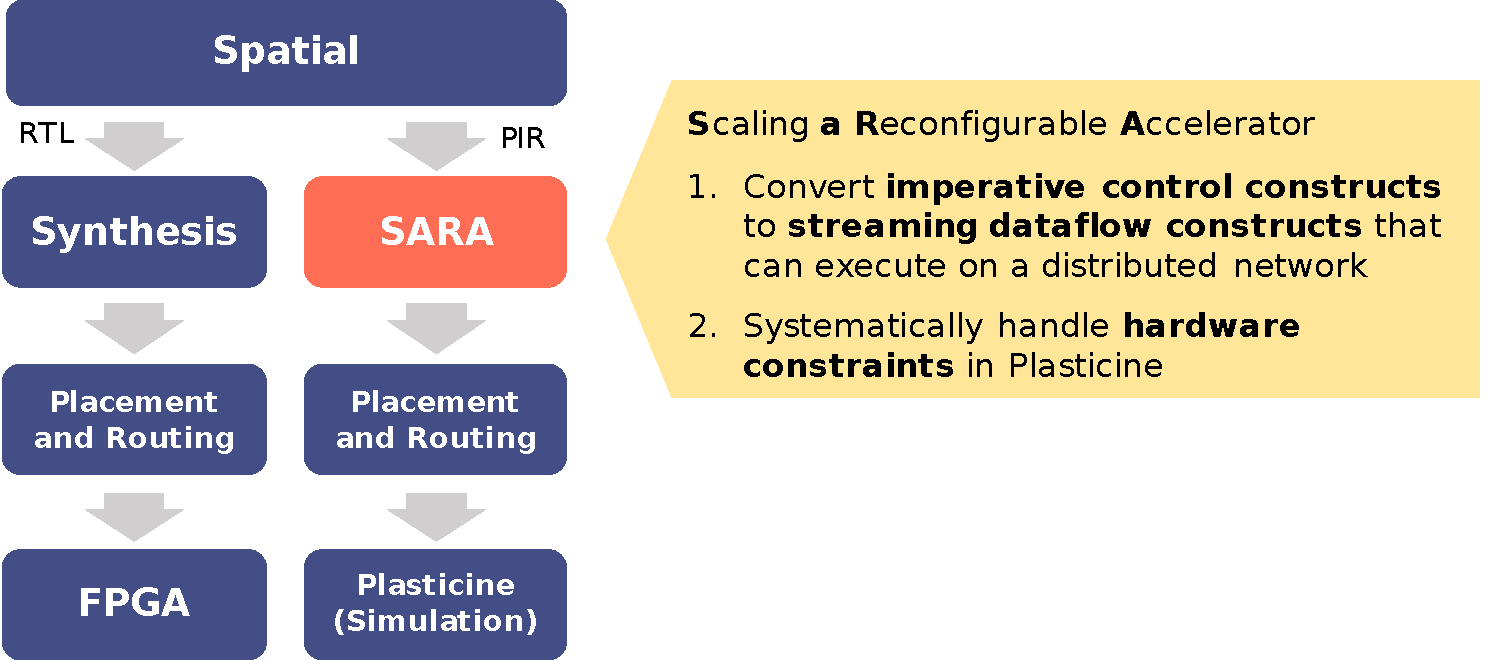
\includegraphics[width=1\textwidth]{figs/spatialstack.pdf}
\caption[Spatial compiler stack to target FPGAs and Plasticine]{
  Spatial compiler stack to target FPGAs and Plasticine
}
\label{fig:spatialstack}
\end{figure*}

Spatial is a target-agnostic language for general reconfigurable architectures. 
The primary targets of Spatial are FPGAs.
Similar to the C-based high-level synthesis languages, such as Vivado HLS~\cite{vivado} and
SDAccel~\cite{sdaccel},
Spatial provides a high-level programming interface that focuses on the algorithmic 
implementations of the application, hiding the low-level hardware interfaces and RTL programming from the
users.
To target Plasticine, we take applications described in Spatial, disabling FPGA-specific
transformations, and perform architecture-specific lowering to \name's IR.
The key transformations we take from the Spatial compiler is loop unrolling, memory buffering, and
memory partitioning
(explained later in \Cref{sec:memsplit}).
Optimizations, such as retiming and scheduling, are disabled for Plasticine, as they cannot be
directly applied.
\Cref{fig:spatialstack} summarizes the compiler flow to target FPGAs and Plasticine from Spatial.

Although \name takes Spatial as the front-end language, \name can be equally
integrated with other imperative languages with similar control constructs, such as C-based high-level
synthesis language, the back-end of the Halide IR~\cite{halide}, the TACO~\cite{taco} compiler, etc.
Nonetheless, using Spatial as our front-end has a few advantages.
Rather than adapting existing languages for processor architectures like most HLS languages, 
Spatial is designed specifically for reconfigurable spatial architectures.
Spatial's language constructs capture the scheduling scheme that can be explored by most
spatial architectures, such as coarse-grained pipelining, streaming dataflow, hierarchical parallelization, 
and finite state machines (FSM).
These language constructs are missing from a processor-based language as they cannot be supported by
a processor.
Spatial IR also differs in its representation of control flow and memory constructs, which are more suitable for analyses of spatial architectures.

Most compilers, such as LLVM~\cite{llvm}, use control flow graphs to represent the control constructs in an imperative program.
The control flow graph implicitly assumes the program is executed in time, which makes it unsuitable
for analysis of a reconfigurable architecture that executes the program in space. 
Instead, Spatial uses a control hierarchy in the IR to capture the scheduling of the program.
The control hierarchy uses a tree structure to represent the nested control constructs, making it
easier to analyze the relations between controllers.
\Cref{fig:spatialegpar} (b) and (c) shows an example of a control flow graph vs. a control hierarchy.
The controller at each level of the hierarchy corresponds to a control construct, such as a loop, or
a branch statement. 
A basic block is attached to each \emph{innermost} controller including instructions
and memory accesses.
If the program has instructions in an outer loop, Spatial automatically inserts a \emph{unit}
controller to wrap the floating instructions.
\name takes the back-end of Spatial IR as input, which is a control hierarchy after loop
unrolling shown in ~\Cref{fig:spatialegpar} (c).

\begin{figure*}
\centering
\begin{subfigure}[b]{0.35\textwidth}
\inputminted{python}{code/spatialegpar.py}
\caption{Pseudo Spatial example}
\end{subfigure}
\hfill
\begin{subfigure}[b]{0.32\textwidth}
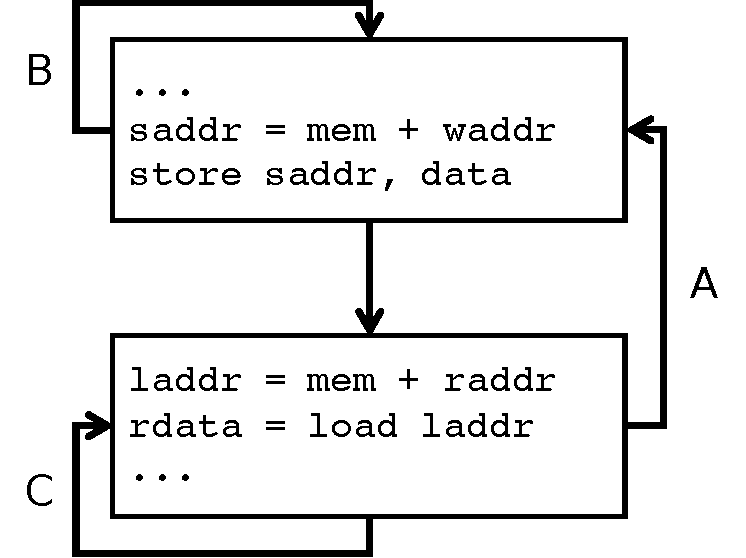
\includegraphics[width=1\textwidth]{figs/controlflow.pdf}
\caption{Control flow graph}
\end{subfigure}
\hfill
\begin{subfigure}[b]{0.25\textwidth}
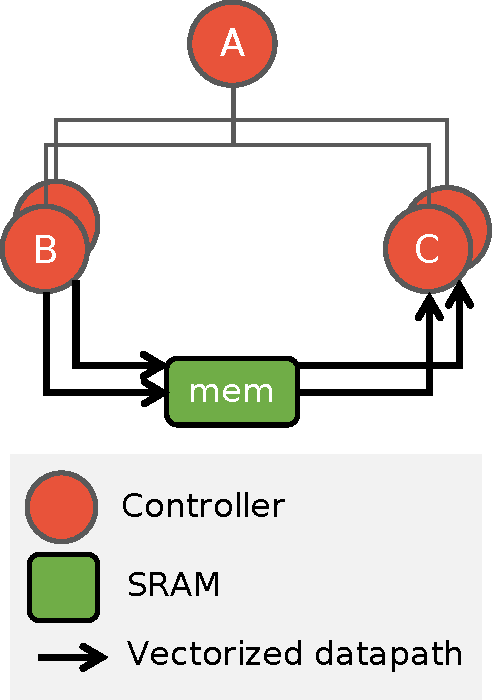
\includegraphics[width=1\textwidth]{figs/spatialir.pdf}
\caption{Schematic Spatial IR}
\end{subfigure}
\caption[Spatial Example]{
  Pseudo example of \name's front-end language.
  (a) shows the an example of \name's front-end language. 
  (b) shows the control-flow graph in traditional CPU-based compiler.
  The `par` keyword indicates outer loop unrolling factor, and
  the `vec` keyword is followed by a inner-loop vectorization factor.
  When an iterator is vectorized, instructions using the vectorized iterator is automatically
  vectorized. When unrolling the outer loop \texttt{A}, the enclosed loop body and
  next-level controllers are duplicated, as suggested in (c).
  Each loop in (a) corresponds to a controller in (c). The inner most controllers \texttt{B} and
  \texttt{C} each contain a basic block within instructions within the inner most loops.
}
\label{fig:spatialegpar}
\end{figure*}

%% Memory model
The representation of data structures in traditional IRs often marries to the memory model of a 
CPU. Traditional compilers, such as LLVM~\cite{llvm}, treat data collections as pointers to a shared
global address space because of the virtual memory abstraction in CPUs.
The hardware, on the back-end, implicitly manage the data movement between an on-chip cache and the off-chip 
memory; this scheme improves programmability of CPU at the cost of hardware complexity and
unpredictable memory
performance.
Accelerators on the other hand often have explicitly managed on-chip scratchpads.
Therefore, modeling data structures as disjoint memory spaces as supposed to pointers is more suitable for reconfigurable architectures.

Spatial is an embedded DSL in Scala.
For simplicity and generality, we will use python-style pseudo code to represent the imperative
input program for the rest of our discussion.
